\begin{figure}[p]
  \centering
  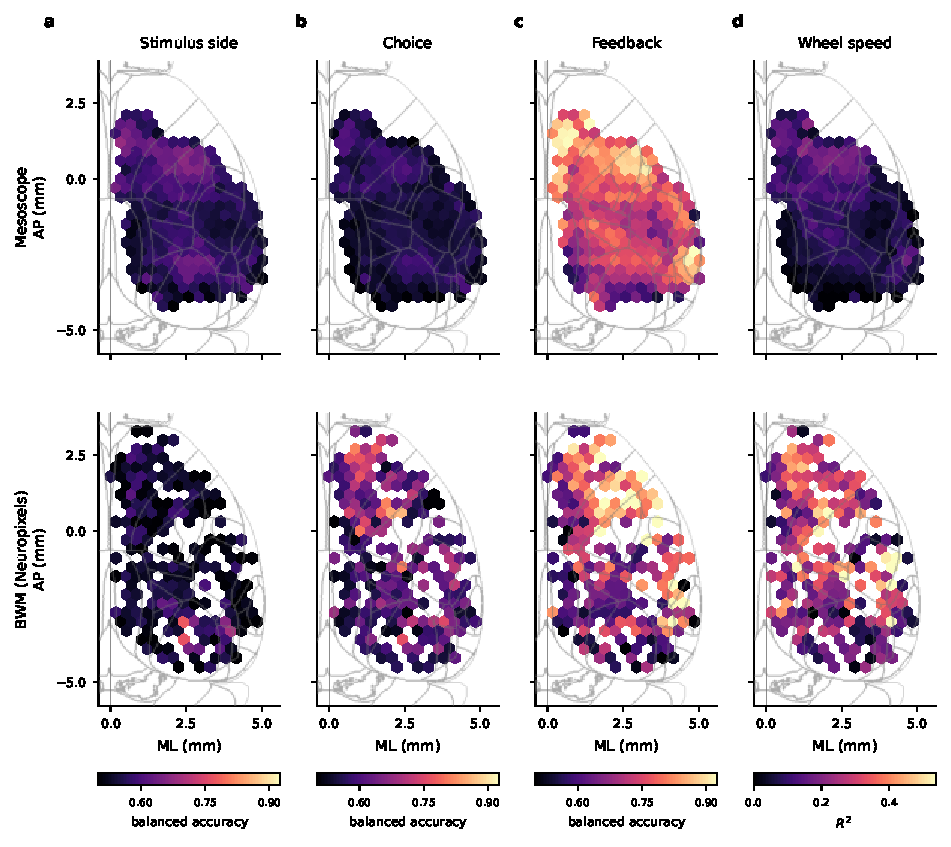
\includegraphics[width=7.00in,height=0.78\textheight,keepaspectratio]{figures/fig6_decoding_all/dorsal_decoding_all_panels.pdf}
  \caption{Dorsal cortex maps, mesoscope two-photon imaging (top row; deconvolved activity of isocortex neurons, canonical sessions) vs Brain Wide Map Neuropixels recordings (bottom row; good isocortex units, 2023 release). Each neuron is assigned to a hexagonal bin (0.4\,mm vertex to vertex) by its medio-lateral (ML) and antero-posterior (AP) Allen CCF position relative to bregma; both hemispheres are folded onto the right one (ML $\to$ $|$ML$|$). Grey lines: Allen top-view region boundaries. Trials: choice made and reaction time 0.08--2\,s (BWM criteria). Colour scales are shared between the two rows. Decoding per session and bin, for every session with $\geq$50 trials and $\geq$10 neurons in the bin: 5-fold stratified cross-validation; binary variables with L2-regularised logistic regression (balanced class weights, regularisation chosen by inner 3-fold cross-validation), wheel speed with ridge regression (penalty chosen by leave-one-out error, folds split by trial). The three binary variables share one colour scale starting at chance (0.5). With all neurons, mesoscope bins hold far more neurons than BWM bins, so scores are not comparable across rows; see the 10-neuron version. \textbf{a} Stimulus side (left vs right, including 0\% contrast) decoded from all neurons of the session in the bin: cross-validated balanced accuracy (chance 0.5), averaged across sessions with $\geq$10 neurons in the bin; activity in the window $[0, 0.1]$\,s (BWM) or $[0, 0.3]$\,s (mesoscope) relative to stimulus onset. \textbf{b} Same for choice (left vs right wheel turn), window $[-0.1, 0]$\,s (BWM) or $[-0.3, 0]$\,s (mesoscope) relative to movement onset. \textbf{c} Same for feedback (reward vs error), window $[0, 0.2]$\,s (BWM) or $[0, 0.3]$\,s (mesoscope) relative to feedback. \textbf{d} Wheel speed (mean absolute wheel velocity) in 0.2\,s bins from $-0.2$ to $1$\,s around movement onset, decoded from the activity in the same bins: cross-validated $R^2$ of ridge regression (chance 0).}
  \label{fig:fig6_decoding_all}
\end{figure}
